\label{JavaAppletCorrectnessKit}
 The main design goals were the following:
 \begin{itemize}
 \item it should provide an easy accessible user interface, that enables average Java programmers to use the tool
 without too much difficulties (in contrast to for example \LOOP). This interface is
described section \ref{Industrialisation};
 \item it should provide a high degree of automation, so that most proof obligations can be discharged without user
 interaction. Only in this way, the tool can be effectively used by non-expert users, which is necessary if we want that
 formal methods will ever be used in industry. 
 \item it should provide high correctness assurance: at the moment the prover says that a certain proof obligation
is satisfied, it should be possible to trust this without any reservation. Nevertheless
the tool is not formally developed, as \LOOP\ is. It implements, in Java, a weakest precondition calculus that
generates lemmas without user interaction. We cannot prove that those lemmas are necessary and sufficient to
ensure the correctness of the applet but the tool is designed in this way;
 \item it should be relatively independent of any particular prover, so that if the use of another prover is
 required (for example by a certification institute) it is relatively easy to adapt the tool accordingly.
\end{itemize}

 This section presents the tool architecture and its principles,
 concerning object-oriented concepts formalization and lemma generation.
\subsubsection{Architecture}
\begin{figure}[tp]
 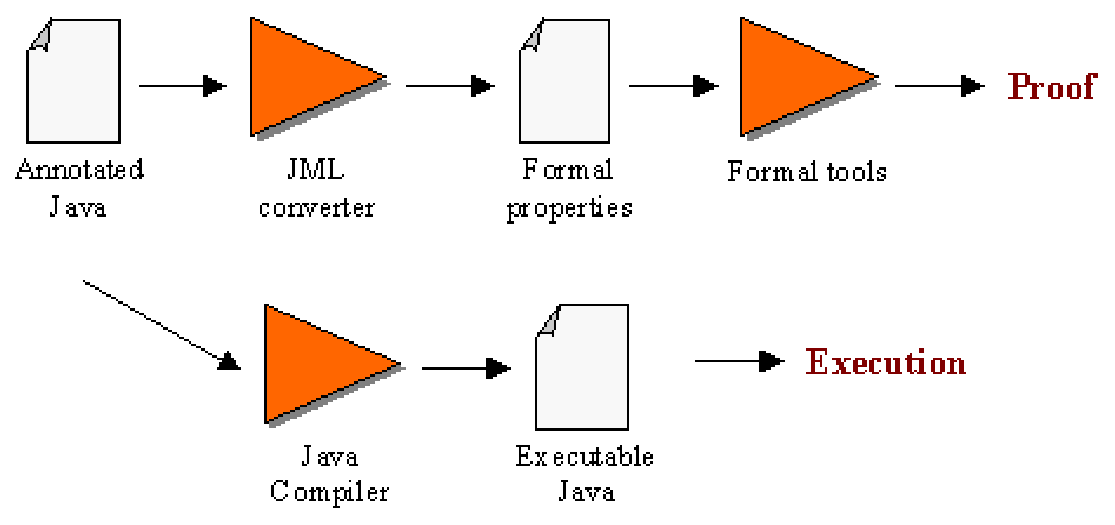
\psfig{file=fm03/image002.eps,width=14cm}
 \caption{\JACK\ architecture}
 \label{JACKarchitecture}
\end{figure}
 Figure \ref{JACKarchitecture} presents an overview of the \JACK\
 architecture.  \JACK\ consists of two parts: a converter (a lemma generator) from
 Java source annotated with JML into JPOL lemmas, and a viewer that
 allows developers to understand the generated
 lemmas.  The viewer is integrated in an IDE and is described more precisely in section
 \ref{Viewer}.  This part focuses on the converter.

 The \JACK\ converter converts a Java class into a JPOL model and allows to
 prove properties. 
 Our goal is to prove properties on source files written with the Java
 language.  To reach this goal, one has to know how to ``translate'' a
 Java source file in formal lemmas.  The two main issues are:
\begin{enumerate}
 \item How to formalize the object-oriented Java features?
 \item How to generate lemmas from Java methods?
\end{enumerate}
The following sections provide answers to those questions.
\subsubsection{Object-oriented concepts formalization}
 The adopted solution concerning the formalization of object-oriented concept is to generate lemmas with the point of
 view of one Java class.
 Each generated lemma for a class contains, as prelude, the formalization of the memory model instantiated with the
context of the current class, i.e. the class hierarchy that it can access, all the fields and methods that it
can use. The prelude contains two parts: a generic one and a contextual one.
 \begin{figure}[thp]
\begin{center}
 $\begin{array}{lllll}
 \rm{SET} & \multicolumn{4}{l}{\rm{REFERENCES}} \\
 \rm{null} & \in & \multicolumn{3}{l}{\rm{REFERENCES}} \\
 \rm{subtypes} & \in & \rm{TYPES} & \leftrightarrow & \rm{TYPES} \\
 \rm{instances} & \subset & \multicolumn{3}{l}{\rm{REFERENCES}} \\
 \rm{null} & \notin & \multicolumn{3}{l}{\rm{instances}} \\
 \rm{typeof} & \in & \rm{instances} & \rightarrow & \rm{TYPES}
 \end{array}$
\end{center}
 \caption{Memory model representation in B}
 \label{Memory model representation}
\end{figure}

 The generic prelude contains many definitions concerning built-in types with their operators.
 It contains also the memory model representation (see Figure \ref{Memory model representation}). This model is defined
 by an infinite set of possible
 references, a particular reference corresponding to $\rm{null}$, a subtyping relation, the set of currently allocated
instances and a function associating a type to each instance.
 This model is completed with definitions allowing to handle arrays that are not given here.
 This set of constants and variables represents the memory state associated to each lemma, corresponding, for instance, to
the state of the memory at the beginning of an operation.
 In this model, an object creation, for instance, will be defined as taking an
arbitrary element from the set of references (different from the special constant null), adding this reference
to the set of instances and assigning a type to it.

 The set of types is defined by $\rm{TYPES} = \rm{NAMES} * \mathbb{N}$, where $\rm{NAMES}$ corresponds to the set of
classes referenced by the program.
 This definition allows to handle the types corresponding to array types: a type corresponds to a class and a
dimension represented by a natural number (for objects, this number is always 0). For instance the Java type
{\tt \rm{Object}} will correspond to the type $\rm{c\_Object} \mapsto 0$ and the Java type {\tt
\rm{Object}[][][]} to $\rm{c\_Object} \mapsto 3$.

 The set $\rm{NAMES}$ is not generic since it depends on the reachable classes from the current one.
 It does not belong to the common prelude but to the contextual one.

 One can notice that primitive types belongs to $\rm{NAMES}$ but they are only used to type arrays. For
instance the Java type {\tt short[]} will correspond to $\rm{c\_short} \mapsto 1$, but the type {\tt short} will
correspond to a prelude-defined type $\rm{t\_short} = -32768..32767$.

The subtyping relation is also valuated depending on the class hierarchy. It assigns to a class itself and all
its subclasses and to an interface itself and all its implementing classes and interfaces.
 This gives, for example,
\begin{center}
$\begin{array}{l}
\rm{subtypes}[\{\rm{c\_RuntimeException} \mapsto 0\}] \\[1 mm]
 = \left\{ \begin{array}{l} \rm{c\_RuntimeException} \mapsto 0,  \\
\rm{c\_NullPointerException} \mapsto 0 , \\ \rm{c\_ArithmeticException} \mapsto 0,   \\
\rm{c\_ArrayIndexOutOfBoundsException} \mapsto 0, \\
\rm{c\_NegativeArraySizeException} \mapsto 0, \\ \rm{c\_ClassCastException} \mapsto 0 , \\
\rm{c\_ArrayStoreException}  \mapsto 0
 \end{array} \right\}
\end{array}$.
\end{center}

 The fields are declared as variables, static fields are directly typed with their translated type,
 member fields are declared as functions from the set of instances of a type to the type of the field.

 The invariants are declared as properties quantified over the instances.

 The drawback of this approach is that one can not directly prove properties on the correctness
 of the formalization.  But, proofs remain simpler as they remain
 centered on the specific case of a dedicated class.
\subsubsection{Lemma generation}
\begin{figure}[p]
 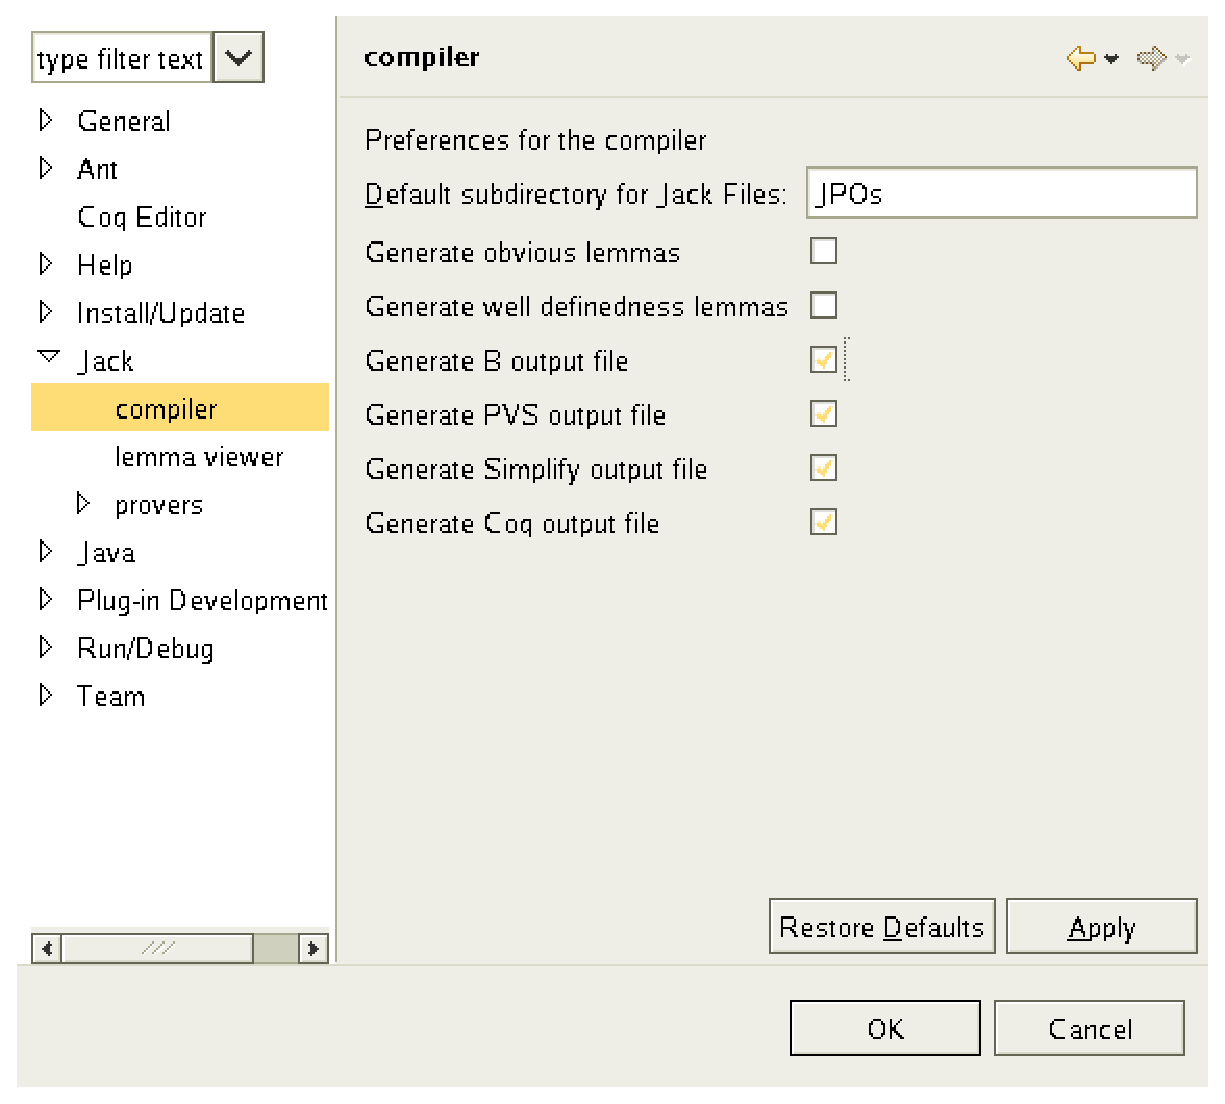
\psfig{file=fm03/preferences-compiler.eps,width=14cm}
 \caption{\JACK\ compiler preferences page}
 \label{JACKcompprefpage}
\end{figure}
 The JML annotations are Java boolean expressions without side
 effects.  Thus, they are easily translated in logical formulas: Java operators are
 translated into functions. For example, shift left (\texttt{<<}) is
 translated into a function associating an integer to a pair of
 integer.  From those translated annotations and the methods code,
 lemmas can be generated automatically.

 From the start, taking into account
 experiences in lemma generation for B machines, we have tried to
 implement a Weakest Precondition (WP) calculus to automate lemma
 generation.  Huisman, in \cite{Huisman:PhD}, presents how the
 classical Hoare logic can be completed to allow the generation of
 lemmas in the context of Java.  The Java statements contain different
 features like control-flow breaks.  So, the classical WP calculus
 should be completed to deal with them.

 Moreover, JML should be lightly upgraded to allow fully automated proof obligation generation.
 Notably, to
 automate lemma generation for the loops, we have had to extend
 the JML language with new keywords: \texttt{loop\_modifies} and \texttt{loop\_exsures}.
 The \texttt{loop\_modifies} keyword allows us to declare the variables modified in
the body of the loop, as it is done for the methods. During the WP calculus, it is necessary to universally
quantify the loop invariant with those variables, and since they cannot be automatically calculated, one has to
specify them.
 The \texttt{loop\_exsures} allows us to specify the exceptional behavior of a loop. It is not necessary to apply
the WP calculus but it can improve the understandability of the specification.

 The two main drawbacks of the WP calculus are the loss of information and
 potential exponentional explosion.  After lemmas have been generated,
 it is often difficult to understand from which part of the code they
 are derived.  To bypass this issue, program flow information is
 associated to each lemma.  This information is used in the viewer
 to associate an execution path to each lemma. This feature is described in the next section.

 Exponentional explosion remains a problem.  Different solutions exist
 to avoid it.  As the WP calculus can be considered as a brute
 force concept, trying to expand all the path of the methods,
 solutions are always based on interaction to reduce this brute force
 by introducing intelligence in the process.

 A simple solution is to require users interaction during lemma
 generation in order to cut unsatisfiable branches.  Rather than introducing
 interaction during generation, another solution is to allow to add
 special annotations in the source code to introduce formulas that are
 taken into account at generation to simplify the lemmas.
 The solution adopted in \JACK\ is to allow to specify blocks. An exponentional explosion usually occurs
in a method with many sequenced branched statement ({\tt if, switch}, etc.) Such methods usually perform
different distinct sequenced treatments.
 Figure \ref{Specified_block} presents the skeleton of such a method. Specifying a block (here the second part
of the method) allows to cut proof obligation generation. This corresponds, in fact, to the simulation of a
method call.
\begin{figure}[htp]
{\tt
\begin{tabbing}
 \hspace{3 cm} \=m()\= \ \{ \\
 \> \> \vdots \\
 \> \> if () \{ $\hdots$ \} \\
 \> \> else \{ $\hdots$ \}   \\
 \> \> \vdots                   \\
 \> \> /*\=@ modifies {\it variables}  \\
 \> \> \> @ ensures {\it property} \\
 \> \> \> @\=*/ \{ \\
 \> \> \> \> \vdots \\
 \> \> \> \> if () \{ $\hdots$ \} \\
 \> \> \> \> else \{ $\hdots$ \}   \\
 \> \> \> \> \vdots                   \\
 \> \> \ \} \\
 \> \> \}
\end{tabbing}
}
 \caption{Specified block}
 \label{Specified_block}
\end{figure}

 With those extensions to the JML language, we are able to obtain a fully automated proof obligation generation.
That is the first step to reach user approval. The second one is to propose an access to those lemmas in a
``Java style'', this is described in the next section.
